\documentclass[11pt,a4paper]{article}

% =========================================================
% PACOTES ESSENCIAIS
% =========================================================
\usepackage[utf8]{inputenc}
\usepackage[T1]{fontenc}
\usepackage[brazilian]{babel}
\usepackage{geometry}
\usepackage{xcolor}
\usepackage{tabularx}
\usepackage{booktabs}
\usepackage{array}
\usepackage{enumitem}
\usepackage{helvet}
\usepackage{ragged2e}
\usepackage{fancyhdr}
\usepackage{lastpage}
\usepackage{url}
\usepackage{cite}
\usepackage{graphicx}
\usepackage{float}
\usepackage{caption}
\usepackage{subcaption}
\usepackage{microtype}
\usepackage[colorlinks=true,linkcolor=primary,citecolor=primary,urlcolor=primary]{hyperref}

% =========================================================
% CORES PERSONALIZADAS E ESTILO
% =========================================================
\definecolor{primary}{RGB}{20, 50, 100}      % Azul marinho acadêmico
\definecolor{secondary}{RGB}{80, 90, 110}    % Cinza ardósia
\definecolor{accent}{RGB}{180, 40, 40}       % Vermelho terracota
\definecolor{lightgray}{RGB}{245, 247, 250}  % Fundo claro
\definecolor{bordergray}{RGB}{210, 215, 225} % Bordas suaves
\definecolor{instructionblue}{RGB}{0,0,255}

\renewcommand{\familydefault}{\sfdefault}

\geometry{
  top=3.35cm,
  bottom=1.8cm,
  left=2.0cm,
  right=2.0cm,
  headheight=64pt,
  headsep=0.45cm
}

\setlength{\parindent}{0pt}
\setlength{\parskip}{0.55em}
\setlist[itemize]{leftmargin=1.5em, itemsep=0.2em}
\setlist[enumerate]{leftmargin=1.5em, itemsep=0.2em}

\newcolumntype{Y}{>{\centering\arraybackslash}X}
\newcolumntype{L}{>{\raggedright\arraybackslash}X}
\newcolumntype{R}{>{\raggedleft\arraybackslash}X}

\AtEndDocument{\label{LastPage}}

% =========================================================
% CAMPOS DO DOCUMENTO
% =========================================================
\newcommand{\NomeProjeto}{Mapa de Calor e Predição do Risco de Acidentes de Trânsito na BR-230}
\newcommand{\VersaoModelo}{1.1}
\newcommand{\DataEmissao}{13/10/2026}

\newcommand{\IntegranteTres}{Winy Gabrielly Soares de Oliveira}
\newcommand{\IntegranteDois}{Ricardo Diniz Mendes}
\newcommand{\IntegranteUm}{João Batista Santos Silva Neto}

\newcommand{\Componentes}{
João Batista Santos Silva Neto \\
Ricardo Diniz Mendes \\
Winy Gabrielly Soares de Oliveira
}

\newcommand{\EmailTres}{winy.soares@discente.ufma.br}
\newcommand{\EmailDois}{ricardo.dm@discente.ufma.br}
\newcommand{\EmailUm}{jbss.neto@discente.ufma.br}

% =========================================================
% CABEÇALHO DO PROJETO (PADRÃO CRISP-DM UFMA)
% =========================================================
\newcommand{\CabecalhoProjeto}{%
\begin{minipage}{\textwidth}
\centering
\renewcommand{\arraystretch}{1.25}

\begin{tabularx}{\textwidth}{|p{2.0cm}|X|p{4.2cm}|}
\hline
& \centering\textbf{Documentação do Projeto}\arraybackslash
& Versão do Modelo: \VersaoModelo \\
\cline{3-3}
& &
Emissão: \DataEmissao
\quad Página: \thepage/\pageref{LastPage} \\
\cline{2-3}
&
\multicolumn{2}{l|}{
Projeto:
\hfill
\textbf{\NomeProjeto}
\hfill
} \\
\hline
\end{tabularx}

\end{minipage}%
}

\pagestyle{fancy}
\fancyhf{}
\fancyhead[C]{\CabecalhoProjeto}
\renewcommand{\headrulewidth}{0pt}
\renewcommand{\footrulewidth}{0pt}

% =========================================================
% ESTILO DAS SEÇÕES
% =========================================================
\makeatletter

\renewcommand\section{
\@startsection{section}{1}{0pt}%
{1.4ex plus .2ex minus .2ex}%
{0.8ex plus .2ex}%
{\normalfont\Large\bfseries\color{primary}}
}

\renewcommand\subsection{
\@startsection{subsection}{2}{0pt}%
{1.2ex plus .2ex minus .2ex}%
{0.6ex plus .2ex}%
{\normalfont\large\bfseries\color{secondary}}
}

\renewcommand\subsubsection{
\@startsection{subsubsection}{3}{0pt}%
{1.0ex plus .2ex minus .2ex}%
{0.5ex plus .2ex}%
{\normalfont\normalsize\bfseries}
}

\makeatother

% =========================================================
% INÍCIO DO DOCUMENTO
% =========================================================
\begin{document}

% ---------------------------------------------------------
% CAPA DO DOCUMENTO
% ---------------------------------------------------------
\begin{center}
\vspace*{1.2cm}

{\Large\textbf{Projeto da Disciplina Ciência de Dados}}\\[0.8em]

{\Large\textbf{Fase 2: Entendimento dos Dados (CRISP-DM)}}

\end{center}

\vspace{0.8cm}
\vfill

\begin{center}

{\Huge\textbf{Relatório de Coleta, Descrição, Exploração e Qualidade dos Dados}}\\[1.5cm]

{\Large\Componentes}\\[1.5cm]

{\Large\textbf{\NomeProjeto}}\\[0.5cm]

\textit{Universidade Federal do Maranhão (UFMA) \\ Programa de Pós-Graduação em Ciência da Computação (PPGCC)}

\end{center}

\vfill
\newpage

% ---------------------------------------------------------
% HISTÓRICO DE REVISÕES
% ---------------------------------------------------------
\section*{Histórico de Revisões do Documento}

\vspace{0.6em}

\begin{center}
\renewcommand{\arraystretch}{1.35}

\begin{tabularx}{\textwidth}{|p{1.6cm}|X|p{3.2cm}|p{2.8cm}|p{2.2cm}|}
\hline
\textbf{Revisão} & \textbf{Descrição} & \textbf{Modificado por} & \textbf{Status} & \textbf{Data} \\
\hline
1.0 & 
Elaboração e consolidação do Relatório da Fase de Entendimento dos Dados (Coleta, Descrição, Exploração e Qualidade), com catálogo de fontes, dicionário com 41 atributos, análises espaciais e temporais na BR-230, e diretrizes para a Preparação dos Dados. & 
Equipe do projeto & 
Concluído & 
13/10/2026 \\
\hline
\end{tabularx}
\end{center}

\newpage

% =========================================================
% 1 COLETA DOS DADOS
% =========================================================
\section{Coleta dos Dados}

A tarefa de coleta inicial (\textit{Collect initial data}) do processo CRISP-DM consiste na aquisição e carga dos conjuntos de dados necessários para a resolução do problema de negócio, registrando seus locais de armazenamento, os métodos empregados para extração e os eventuais obstáculos técnicos superados~\cite{chapman2000}. O objetivo central do projeto é a construção de um mapa de calor e a predição da gravidade do risco de acidentes na rodovia federal BR-230 (Rodovia Transamazônica).

Para atender a essas metas, foram coletados os registros históricos de acidentes rodoviários do ano de 2025 disponibilizados publicamente pela Polícia Rodoviária Federal (PRF)~\cite{prfdados}. As extrações governamentais apresentam diferentes granularidades de dados, complementadas por fontes oficiais de validação externa: o Anuário Estatístico 2025 da PRF~\cite{prfanuario2025} e o cadastro oficial da malha rodoviária federal mantido pelo DNIT~\cite{dnit2026}.

\subsection{Automação de Download e Série Histórica Pós-Pandemia (2022 a 2025)}

Em consonância com as diretrizes de reprodutibilidade científica e o plano de contingência formulado na Fase de Negócio, o projeto implementa rotinas automáticas de download e extração diretamente a partir dos repositórios oficiais da PRF (via Google Drive institucional). Se o arquivo de qualquer ano não estiver presente na pasta local \texttt{bases/}, o pipeline efetua a requisição e descompactação automática, sem necessidade de download manual.

\textbf{Definição do Período Pós-Pandemia:} Foram consolidados os dados do quadriênio \textbf{2022 a 2025}. Os anos de 2020 e 2021 foram descartados devido às anomalias severas de circulação e restrições sanitárias decorrentes da pandemia de COVID-19. A Tabela~\ref{tab:pos_pandemia} resume a evolução da série histórica na rodovia BR-230.

\begin{table}[H]
\centering
\small
\renewcommand{\arraystretch}{1.2}
\caption{Evolução dos acidentes e letalidade na BR-230 no quadriênio pós-pandemia (2022 a 2025).}
\label{tab:pos_pandemia}
\begin{tabularx}{\textwidth}{|c|c|c|c|c|c|}
\hline
\textbf{Ano} & \textbf{Acidentes (Brasil)} & \textbf{Acidentes (BR-230)} & \textbf{Mortos (BR-230)} & \textbf{Fatais (BR-230)} & \textbf{Letalidade (\%)} \\
\hline
2022 & 64.606 & 1.345 & 148 & 135 & 10,04\% \\
\hline
2023 & 67.766 & 1.403 & 160 & 143 & 10,19\% \\
\hline
2024 & 73.202 & 1.724 & 175 & 157 & 9,11\% \\
\hline
2025 & 72.529 & 1.745 & 192 & 168 & 9,63\% \\
\hline
\textbf{Total} & \textbf{278.103} & \textbf{6.217} & \textbf{675} & \textbf{603} & \textbf{9,70\%} \\
\hline
\end{tabularx}
\end{table}

A consolidação do quadriênio acumula \textbf{6.217 acidentes} e \textbf{603 sinistros fatais} na BR-230, estabilizando as amostras dos estados com menor densidade populacional (Ceará atinge 82 acidentes, Tocantins 74 e Amazonas 92) e viabilizando a divisão temporal prospectiva para modelagem preditiva (treinamento em 2022--2024 e teste prospectivo em 2025).

\subsection{Catálogo Consolidado de Fontes de Dados}

A Tabela~\ref{tab:catalogo} apresenta o catálogo consolidado das bases adquiridas, registrando o formato, a unidade de análise (grão), as dimensões na escala nacional e no recorte da BR-230, o consumo em disco e a função técnica desempenhada no pipeline analítico.

\begin{table}[H]
\centering
\small
\renewcommand{\arraystretch}{1.25}
\caption{Catálogo das fontes de dados adquiridas para o projeto.}
\label{tab:catalogo}
\begin{tabularx}{\textwidth}{|p{2.6cm}|p{2.5cm}|p{1.8cm}|p{2.3cm}|p{2.0cm}|X|}
\hline
\textbf{Fonte / Autor} & \textbf{Arquivo} & \textbf{Formato} & \textbf{Grão} & \textbf{Volume BR-230} & \textbf{Papel no Projeto} \\
\hline
Polícia Rodoviária Federal (PRF) & \texttt{datatran2025.csv} & CSV (\textit{latin-1}) & 1 linha = 1 ocorrência & 1.745 acidentes (21,1 MB nac.) & Mapa de Calor, coordenadas espaciais, sazonalidade e desfecho de gravidade. \\
\hline
Polícia Rodoviária Federal (PRF) & \texttt{acidentes2025.csv} & CSV (\textit{latin-1}) & 1 linha = 1 pessoa & 4.410 pessoas (72,8 MB nac.) & Perfil demográfico de vítimas, condutores, veículos e gravidade clínica. \\
\hline
Polícia Rodoviária Federal (PRF) & \texttt{acidentes2025\_ todas\_causas\_ tipos.csv} & CSV (\textit{latin-1}) & 1 linha = pessoa $\times$ causa $\times$ tipo & 18.255 linhas (~195 MB nac.) & Mapeamento de causas secundárias e multiplicidade de tipos de sinistros. \\
\hline
PRF (Oficial) & \textit{Anuário Estatístico 2025} & PDF / Relatório & Agregado nacional / UF & 72.529 sinistros, 6.043 óbitos & Validação externa de fidelidade dos dados brutos locais. \\
\hline
DNIT & \textit{Malha Rodoviária} & Especificação cadastral & Segmento de rodovia & 4.260 km totais (PB: 521 km) & Delimitação territorial e validação dos marcos quilométricos. \\
\hline
\end{tabularx}
\end{table}

\subsection{Fonte A: PRF --- Acidentes Agrupados por Ocorrência (\texttt{datatran2025.csv})}

O arquivo \texttt{datatran2025.csv} é a fonte principal do estudo. Nele, cada registro representa exatamente um acidente de trânsito em rodovia federal com boletim de ocorrência lavrado no decorrer do ano de 2025.
\begin{itemize}
    \item \textbf{Localização e Acesso:} Armazenado no diretório local \texttt{bases/datatran2025.csv}, obtido por download via protocolo HTTP no Portal Brasileiro de Dados Abertos (\url{https://www.gov.br/prf/pt-br/acesso-a-informacao/dados-abertos/dados-abertos-da-prf}).
    \item \textbf{Volume Bruto e Recorte:} O arquivo possui 72.529 linhas e 30 colunas na escala nacional (21,1 MB em disco). O filtro pela rodovia de interesse (\texttt{br == 230}) extrai 1.745 acidentes.
    \item \textbf{Uso no Projeto:} Alimenta o Mapa de Calor através do par de coordenadas geográficas (\texttt{latitude} e \texttt{longitude}), suporta as agregações temporais (mês, dia da semana, faixa horária, fase do dia) e define a severidade da ocorrência.
\end{itemize}

\subsection{Fonte B: PRF --- Acidentes Agrupados por Pessoa (\texttt{acidentes2025.csv})}

O arquivo \texttt{acidentes2025.csv} detalha o perfil individual de cada cidadão envolvido no evento de trânsito.
\begin{itemize}
    \item \textbf{Localização e Acesso:} Diretório \texttt{bases/acidentes2025.csv}, obtido diretamente do portal da PRF.
    \item \textbf{Volume Bruto e Recorte:} Possui 194.629 linhas e 35 colunas (72,8 MB em disco). No recorte da BR-230, soma 4.410 linhas de pessoas vinculadas aos 1.745 sinistros.
    \item \textbf{Uso no Projeto:} Permite construir o perfil de vítimas (idade, gênero, condição física), de condutores, pedestres e passageiros, além de caracterizar a frota de veículos envolvida (tipo de veículo, marca, ano de fabricação).
\end{itemize}

\subsection{Fonte C: PRF --- Todas as Causas e Tipos (\texttt{acidentes2025\_todas\_causas\_tipos.csv})}

Esta extração desdobra as ocorrências em todas as causas prováveis e dinâmicas de impacto apontadas pelos agentes policiais.
\begin{itemize}
    \item \textbf{Volume e Processamento:} O arquivo nacional atinge 584.010 linhas e 37 colunas (~195 MB). Pelo seu volume elevado, sua carga foi processada via blocos iterativos (\textit{chunksize} de 200.000 linhas), isolando 18.255 registros referentes à BR-230.
    \item \textbf{Uso no Projeto:} Identificação de causas secundárias e tipos associados. O estudo demonstrou que 42,5\% dos sinistros da BR-230 possuem mais de uma causa registrada e 65,5\% possuem mais de um tipo de ocorrência. Quando filtrado para causa principal e tipo de ordem 1, o conjunto colapsa perfeitamente para as 4.410 linhas do arquivo por pessoa, confirmando a integridade do modelo relacional da PRF.
\end{itemize}

\subsection{Fontes Externas de Validação}

Para garantir que a base local é autêntica e represents o fechamento consolidado do ano de 2025, foram incorporadas duas referências institucionais:
\begin{enumerate}
    \item \textbf{Anuário Estatístico 2025 da PRF:} Relatório oficial consolidado em maio de 2026 contendo os totais de sinistros, feridos e óbitos no país e por rodovia.
    \item \textbf{Dados Cadastrais do DNIT:} Atestam a extensão de 4.260 km da BR-230 e os limites oficiais de cada trecho estadual (ex.: 521,0 km na Paraíba e 144,7 km no Tocantins).
\end{enumerate}

\subsection{Problemas Encontrados na Coleta e Resoluções Técnicas}

Durante a ingestão inicial dos dados, três problemas técnicos relevantes foram diagnosticados e solucionados:
\begin{enumerate}
    \item \textbf{Codificação dos Arquivos (\textit{Encoding}):} Os arquivos exportados pela PRF encontram-se codificados em \texttt{ISO-8859-1} (\textit{latin-1}). A leitura sob padrão \texttt{UTF-8} resulta em falhas de decodificação. A rotina de carga foi configurada com o parâmetro explícito \texttt{encoding='latin-1'}, preservando integralmente acentuações e caracteres especiais.
    \item \textbf{Delimitadores e Separador Decimal:} Os dados utilizam ponto e vírgula (\texttt{;}) como separador de campos e vírgula (\texttt{,}) como separador decimal para latitude, longitude e quilometragem. A leitura inadvertida converte essas grandezas em texto (\textit{string}). Configurou-se \texttt{sep=';'} e \texttt{decimal=','}, garantindo que as coordenadas fossem carregadas como números de ponto flutuante de precisão dupla (\texttt{float64}).
    \item \textbf{Multiplicação Granular no Arquivo Expandido:} O arquivo de todas as causas e tipos repete o mesmo acidente em múltiplas linhas. Se utilizado ingenuamente para contagem de acidentes, superestimaria as ocorrências na BR-230 em mais de 10 vezes (18.255 linhas vs. 1.745 acidentes reais). Definiu-se como regra arquitetural o uso exclusivo de \texttt{datatran2025.csv} para a contagem de sinistros e alimentação do mapa de calor.
\end{enumerate}

\newpage

% =========================================================
% 2 DESCRIÇÃO DOS DADOS
% =========================================================
\section{Descrição dos Dados}

A tarefa de descrição (\textit{Describe data}) visa inspecionar a superfície dos dados adquiridos, relatando a quantidade de registros e campos, alocação de memória RAM, delimitação temporal, a identidade das variáveis e a avaliação do atendimento aos requisitos de negócio.

\subsection{Embalagem e Propriedades de Superfície}

A Tabela~\ref{tab:embalagem} resume as propriedades de superfície e consumo computacional dos arquivos carregados em memória.

\begin{table}[H]
\centering
\small
\renewcommand{\arraystretch}{1.25}
\caption{Resumo da embalagem (\textit{packaging}) dos arquivos na escala nacional.}
\label{tab:embalagem}
\begin{tabularx}{\textwidth}{|X|c|c|c|c|p{3.2cm}|}
\hline
\textbf{Arquivo / Recorte} & \textbf{Linhas (Nac.)} & \textbf{Colunas} & \textbf{BR-230} & \textbf{Memória RAM} & \textbf{Formato} \\
\hline
\texttt{datatran2025.csv} & 72.529 & 30 & 1.745 & 82,5 MB & CSV (\textit{latin-1}, sep \texttt{;}) \\
\hline
\texttt{acidentes2025.csv} & 194.629 & 35 & 4.410 & 279,3 MB & CSV (\textit{latin-1}, sep \texttt{;}) \\
\hline
\textbf{Série BR-230 (2022--2025)} & \textbf{278.103} & \textbf{30} & \textbf{6.217} & \textbf{315,2 MB} & CSV (\textit{latin-1}, sep \texttt{;}) \\
\hline
\textbf{Pessoas BR-230 (2022--2025)} & \textbf{766.412} & \textbf{35} & \textbf{15.764} & \textbf{1.085 MB} & CSV (\textit{latin-1}, sep \texttt{;}) \\
\hline
\texttt{acidentes2025\_expandido} & 584.010 & 37 & 18.255 & ~750 MB (streaming) & CSV (\textit{latin-1}, sep \texttt{;}) \\
\hline
\end{tabularx}
\end{table}

Nota-se uma correspondência biunívoca perfeita: os 72.529 identificadores de acidente presentes em \texttt{datatran2025.csv} encontram correspondência exata nos outros dois arquivos, sem nenhum registro órfão.

\subsection{Delimitação Temporal (Início e Fim da Base)}

A base cobre com continuidade os 12 meses do ano de 2025:
\begin{itemize}
    \item \textbf{Primeiro registro observado:} 01/01/2025 às 06:20:00 (ID 652493).
    \item \textbf{Último registro observado:} 31/12/2025 às 23:55:00 (ID 757510).
    \item Na escala nacional, o volume mensal varia de 5.287 (fevereiro) a 6.788 ocorrências (dezembro). No recorte da BR-230, as ocorrências oscilam de forma equilibrada entre 120 e 166 casos mensais.
\end{itemize}

\subsection{Grão e Relacionamento de Integridade}

No arquivo por pessoa (\texttt{acidentes2025.csv}), as variáveis \texttt{ilesos}, \texttt{feridos\_leves}, \texttt{feridos\_graves} e \texttt{mortos} funcionam como \textit{flags} indicadoras binárias (0 ou 1) atribuídas ao indivíduo daquela linha. A soma dessas colunas agrupada pelo identificador \texttt{id} recupera de maneira exata o total de vítimas computado nas colunas homônimas em \texttt{datatran2025.csv}.

\subsection{Dicionário de Dados Consolidado}

A Tabela~\ref{tab:dicionario} cataloga as 41 variáveis que integram o ecossistema de dados da PRF, indicando tipo primitivo, grão de origem e significado semântico.

\begin{table}[H]
\centering
\scriptsize
\renewcommand{\arraystretch}{1.2}
\caption{Dicionário de dados consolidado das fontes da PRF (41 variáveis).}
\label{tab:dicionario}
\begin{tabularx}{\textwidth}{|p{2.8cm}|p{1.2cm}|p{2.3cm}|X|}
\hline
\textbf{Campo} & \textbf{Tipo} & \textbf{Grão / Arquivo} & \textbf{Descrição Semântica / Domínio} \\
\hline
\texttt{id} & \texttt{int64} & Ocorrência e Pessoa & Identificador numérico único do acidente rodoviário. \\
\hline
\texttt{pesid} & \texttt{int64} & Pessoa e Expandido & Identificador único da pessoa. O valor 0 indica pessoa não identificada. \\
\hline
\texttt{data\_inversa} & \texttt{str} & Ocorrência & Data do acidente no formato AAAA-MM-DD (2025-01-01 a 2025-12-31). \\
\hline
\texttt{dia\_semana} & \texttt{str} & Ocorrência & Dia da semana por extenso (segunda-feira a domingo). \\
\hline
\texttt{horario} & \texttt{str} & Ocorrência & Horário de ocorrência no formato HH:MM:SS (00:00:00 a 23:59:59). \\
\hline
\texttt{uf} & \texttt{str} & Ocorrência & Unidade da Federação do local do sinistro (PB, PA, MA, PI, AM, CE, TO). \\
\hline
\texttt{br} & \texttt{int64} & Ocorrência & Número identificador da rodovia federal (230 no recorte do estudo). \\
\hline
\texttt{km} & \texttt{float64} & Ocorrência & Marco quilométrico na rodovia (a contagem reinicia em cada UF). \\
\hline
\texttt{municipio} & \texttt{str} & Ocorrência & Município de ocorrência do fato. \\
\hline
\texttt{causa\_acidente} & \texttt{str} & Ocorrência e Expandido & Causa registrada pelo policial (causa principal em \texttt{datatran}). \\
\hline
\texttt{tipo\_acidente} & \texttt{str} & Ocorrência e Expandido & Dinâmica do impacto (tipo de ordem 1 em \texttt{datatran}). \\
\hline
\texttt{classificacao\_acidente} & \texttt{str} & Ocorrência & Gravidade: Sem Vítimas, Com Vítimas Feridas ou Com Vítimas Fatais. \\
\hline
\texttt{fase\_dia} & \texttt{str} & Ocorrência & Luminosidade: Pleno dia, Plena Noite, Anoitecer ou Amanhecer. \\
\hline
\texttt{sentido\_via} & \texttt{str} & Ocorrência & Direção do fluxo: Crescente, Decrescente ou Não Informado. \\
\hline
\texttt{condicao\_metereologica}& \texttt{str} & Ocorrência & Condição meteorológica registrada no momento do boletim. \\
\hline
\texttt{tipo\_pista} & \texttt{str} & Ocorrência & Perfil transversal: Simples, Dupla ou Múltipla. \\
\hline
\texttt{tracado\_via} & \texttt{str} & Ocorrência & Geometria da pista (pode conter valores compostos com ponto e vírgula). \\
\hline
\texttt{uso\_solo} & \texttt{str} & Ocorrência & Ambiente circundante: Sim (área urbana) ou Não (área rural). \\
\hline
\texttt{pessoas} & \texttt{int64} & Ocorrência & Quantidade total de pessoas envolvidas no sinistro. \\
\hline
\texttt{mortos} & \texttt{int64} & Ocorrência / Pessoa & Na ocorrência: total de óbitos; na pessoa: indicador binário (0/1). \\
\hline
\texttt{feridos\_leves} & \texttt{int64} & Ocorrência / Pessoa & Na ocorrência: contagem; na pessoa: indicador binário (0/1). \\
\hline
\texttt{feridos\_graves} & \texttt{int64} & Ocorrência / Pessoa & Na ocorrência: contagem; na pessoa: indicador binário (0/1). \\
\hline
\texttt{ilesos} & \texttt{int64} & Ocorrência / Pessoa & Na ocorrência: contagem; na pessoa: indicador binário (0/1). \\
\hline
\texttt{ignorados} & \texttt{int64} & Ocorrência & Vítimas com estado físico indeterminado no atendimento. \\
\hline
\texttt{feridos} & \texttt{int64} & Ocorrência & Soma aritmética de feridos leves e graves. \\
\hline
\texttt{veiculos} & \texttt{int64} & Ocorrência & Quantidade de veículos automotores envolvidos. \\
\hline
\texttt{latitude} & \texttt{float64} & Ocorrência & Coordenada de latitude em graus decimais (Datum WGS84). \\
\hline
\texttt{longitude} & \texttt{float64} & Ocorrência & Coordenada de longitude em graus decimais (Datum WGS84). \\
\hline
\texttt{regional} & \texttt{str} & Ocorrência & Superintendência Regional da PRF responsável pelo boletim. \\
\hline
\texttt{delegacia} & \texttt{str} & Ocorrência & Delegacia da PRF responsável pela circunscrição. \\
\hline
\texttt{uop} & \texttt{str} & Ocorrência & Unidade Operacional Policial da PRF. \\
\hline
\texttt{id\_veiculo} & \texttt{int64} & Pessoa & Identificador do veículo associado à pessoa. \\
\hline
\texttt{tipo\_veiculo} & \texttt{str} & Pessoa & Categoria do veículo (Motocicleta, Automóvel, Caminhão, etc.). \\
\hline
\texttt{marca} & \texttt{str} & Pessoa & Fabricante e modelo comercial do veículo. \\
\hline
\texttt{ano\_fabricacao\_veiculo}& \texttt{int64} & Pessoa & Ano fabril do veículo (o valor 0 indica ausência de informação). \\
\hline
\texttt{tipo\_envolvido} & \texttt{str} & Pessoa & Condutor, passageiro, pedestre, cavaleiro ou testemunha. \\
\hline
\texttt{estado\_fisico} & \texttt{str} & Pessoa & Condição clínica: Ileso, Lesões Leves, Lesões Graves ou Óbito. \\
\hline
\texttt{idade} & \texttt{int64} & Pessoa & Idade em anos completos (0 opera como omissão). \\
\hline
\texttt{sexo} & \texttt{str} & Pessoa & Sexo declarado: Masculino, Feminino ou Não Informado. \\
\hline
\texttt{causa\_principal} & \texttt{str} & Expandido & Flag indicadora se a linha é a causa principal (Sim/Não). \\
\hline
\texttt{ordem\_tipo\_acidente} & \texttt{int64} & Expandido & Ordem sequencial do impacto na colisão (iniciando em 1). \\
\hline
\end{tabularx}
\end{table}

\subsection{Resumo Estatístico de Superfície}

A Tabela~\ref{tab:resumo_numerico} confronta as estatísticas de variáveis numéricas entre a base nacional e o recorte da BR-230.

\begin{table}[H]
\centering
\small
\renewcommand{\arraystretch}{1.2}
\caption{Resumo univariado das variáveis contínuas e discretas (Recorte BR-230: $n=1.745$).}
\label{tab:resumo_numerico}
\begin{tabularx}{\textwidth}{|p{2.8cm}|c|c|c|c|c|c|c|}
\hline
\textbf{Atributo} & \textbf{Média} & \textbf{Desvio Pad.} & \textbf{Mínimo} & \textbf{Q25} & \textbf{Mediana} & \textbf{Q75} & \textbf{Máximo} \\
\hline
\texttt{km} & 179,9 km & 240,6 km & 0,0 km & 25,0 km & 78,0 km & 231,0 km & 1.230,0 km \\
\hline
\texttt{pessoas} & 2,46 & 1,82 & 1,00 & 2,00 & 2,00 & 3,00 & 45,00 \\
\hline
\texttt{veiculos} & 1,67 & 0,81 & 1,00 & 1,00 & 2,00 & 2,00 & 11,00 \\
\hline
\texttt{mortos} & 0,110 & 0,39 & 0,00 & 0,00 & 0,00 & 0,00 & 4,00 \\
\hline
\texttt{feridos\_leves} & 0,79 & 1,05 & 0,00 & 0,00 & 1,00 & 1,00 & 25,00 \\
\hline
\texttt{feridos\_graves} & 0,35 & 0,68 & 0,00 & 0,00 & 0,00 & 1,00 & 7,00 \\
\hline
\texttt{ilesos} & 0,91 & 1,32 & 0,00 & 0,00 & 1,00 & 1,00 & 40,00 \\
\hline
\texttt{latitude} & -6,71$^\circ$ & 1,94$^\circ$ & -9,75$^\circ$ & -7,21$^\circ$ & -7,09$^\circ$ & -7,04$^\circ$ & -2,32$^\circ$ \\
\hline
\texttt{longitude} & -40,32$^\circ$ & 7,85$^\circ$ & -64,95$^\circ$ & -35,88$^\circ$ & -35,32$^\circ$ & -34,88$^\circ$ & -34,83$^\circ$ \\
\hline
\end{tabularx}
\end{table}

A taxa média de óbitos por sinistro na BR-230 (0,110) é 32,5\% superior à média nacional (0,083), confirmando a criticidade da rodovia. O terceiro quartil do marco quilométrico (231,0 km) indica forte assimetria: mais de 75\% dos sinistros ocorrem nos segmentos iniciais de cada estado.

\subsection{Avaliação de Atendimento aos Requisitos}

O exame dos dados confirma a aderência aos requisitos definidos na Fase 1:
\begin{itemize}
    \item \textbf{Requisito de Representação Espacial:} 100\% dos acidentes da BR-230 possuem coordenadas válidas de latitude e longitude, aptas à geração de Mapas de Calor por Estimação de Densidade Kernel (KDE)~\cite{le2020}.
    \item \textbf{Requisito Temporal e Viário:} Data, horário, perfil da pista, uso do solo e condição meteorológica possuem preenchimento integral, fornecendo as variáveis explicativas do componente preditivo.
    \item \textbf{Requisito de Desfecho Supervisionado:} A variável \texttt{classificacao\_acidente} encontra-se 100\% preenchida no recorte, com 168 acidentes com vítimas fatais (9,63\%) e 1.329 com feridos (76,16\%).
\end{itemize}

\newpage

% =========================================================
% 3 EXPLORAÇÃO DOS DADOS (EDA)
% =========================================================
\section{Exploração dos Dados}

A exploração estatística e visual dos dados (\textit{Explore data}) responde a cinco questões analíticas centrais estabelecidas para guiar a mineração de dados.

\subsection{Questão 1: Concentração e Distribuição Espacial na BR-230}

\textit{Os acidentes cobrem o corredor da BR-230? Em quais estados, municípios e trechos os sinistros se acumulam?}

A BR-230 estende-se da costa oriental paraibana até o sudoeste do Amazonas. Em 2025, a PRF registrou acidentes em 7 Unidades da Federação e 93 municípios. A Tabela~\ref{tab:uf_br230} sintetiza a distribuição das ocorrências por estado.

\begin{table}[H]
\centering
\small
\renewcommand{\arraystretch}{1.2}
\caption{Distribuição consolidada de acidentes e gravidade por UF na BR-230 (2022--2025).}
\label{tab:uf_br230}
\begin{tabularx}{\textwidth}{|c|c|c|c|c|c|c|c|}
\hline
\textbf{UF} & \textbf{Acidentes} & \textbf{Part. (\%)} & \textbf{Mortos} & \textbf{Feridos} & \textbf{Km Máx.} & \textbf{Fatais} & \textbf{Prop. Fatais (\%)} \\
\hline
\textbf{PB} & 4.244 & 68,26\% & 280 & 4.949 & 521,0 km & 247 & 5,82\% \\
\hline
\textbf{PA} & 1.000 & 16,08\% & 187 & 1.013 & 1.230,0 km & 170 & 17,00\% \\
\hline
\textbf{MA} & 430 & 6,92\% & 95 & 485 & 570,0 km & 86 & 20,00\% \\
\hline
\textbf{PI} & 295 & 4,75\% & 46 & 337 & 310,4 km & 42 & 14,24\% \\
\hline
\textbf{AM} & 92 & 1,48\% & 8 & 108 & 687,0 km & 6 & 6,52\% \\
\hline
\textbf{CE} & 82 & 1,32\% & 41 & 78 & 113,0 km & 36 & 43,90\% \\
\hline
\textbf{TO} & 74 & 1,19\% & 18 & 104 & 144,7 km & 16 & 21,62\% \\
\hline
\textbf{Total} & \textbf{6.217} & \textbf{100,0\%} & \textbf{675} & \textbf{7.074} & --- & \textbf{603} & \textbf{9,70\%} \\
\hline
\end{tabularx}
\end{table}

A Figura~\ref{fig:mapa_espacial} ilustra a dispersão espacial das coordenadas de latitude e longitude dos 1.745 acidentes, evidenciando o corredor da Transamazônica colorido pela gravidade da ocorrência.

\begin{figure}[H]
\centering
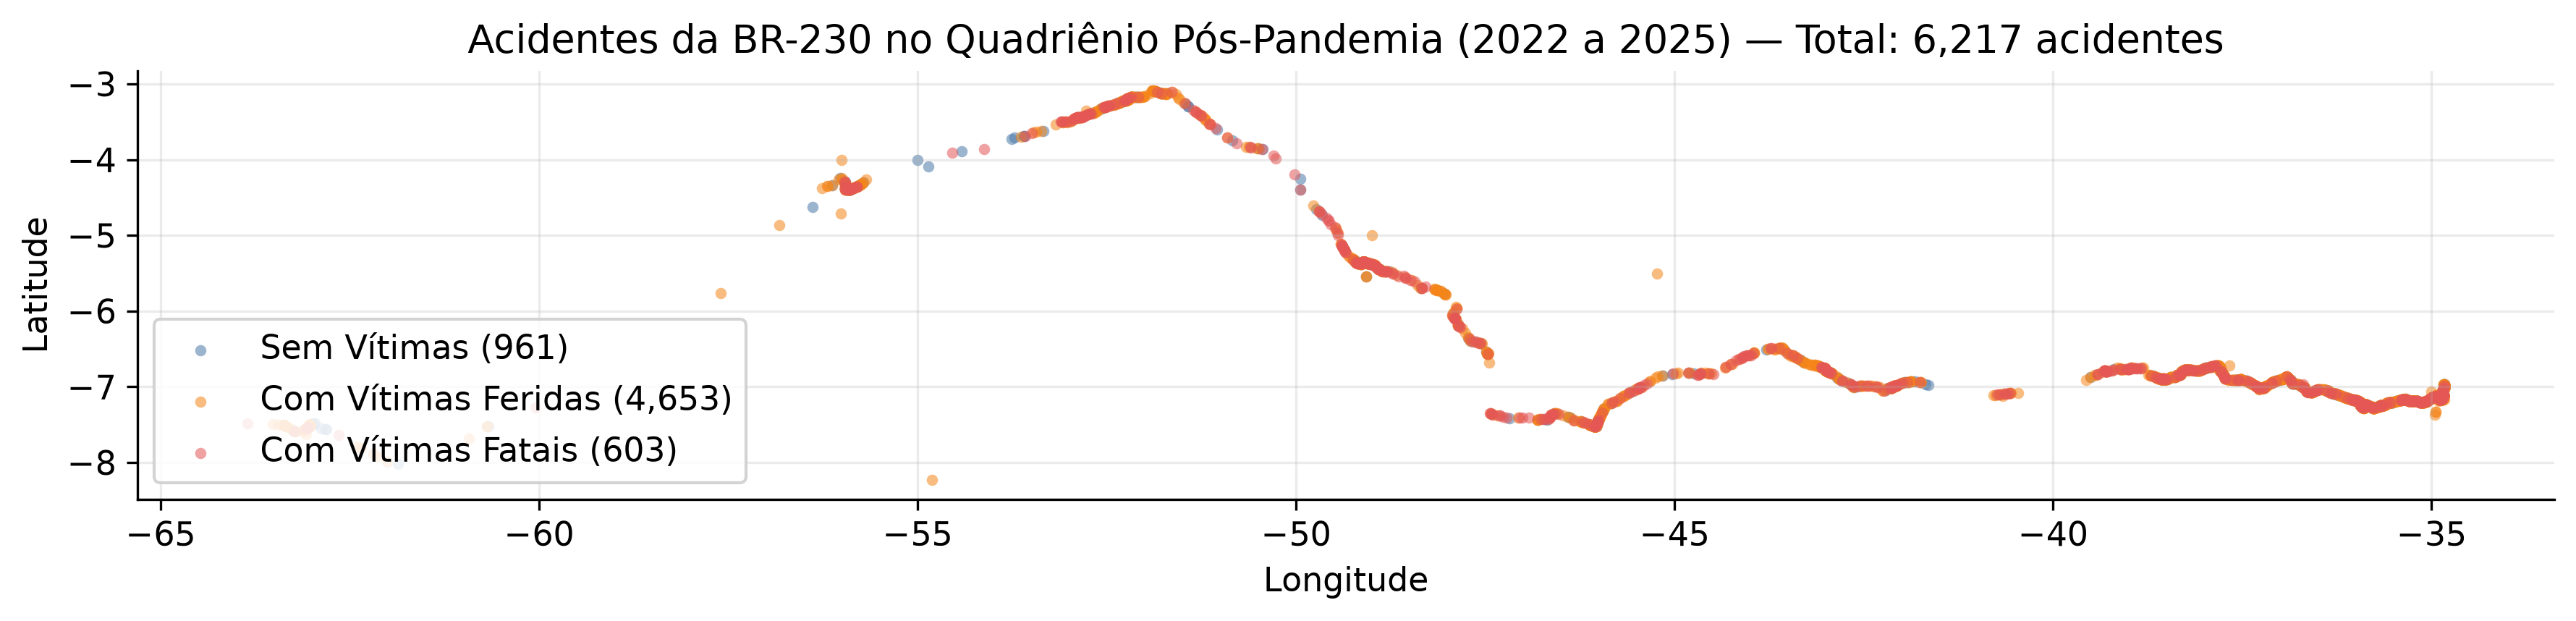
\includegraphics[width=0.95\textwidth]{figuras/mapa_dispersao_br230.png}
\caption{Distribuição espacial dos acidentes ao longo da BR-230 no quadriênio pós-pandemia (2022 a 2025, N = 6.217), discriminados por gravidade.}
\label{fig:mapa_espacial}
\end{figure}

A análise em janelas de 50 km revelou que a faixa do \textbf{km 0 ao km 50 na Paraíba} concentra isoladamente \textbf{2.095 acidentes} (33,7\% do total da rodovia no país ao longo de 2022--2025), compreendendo a área metropolitana de João Pessoa, Cabedelo, Bayeux e Santa Rita. Todavia, a proporção de acidentes fatais nessa faixa é de apenas \textbf{3,10\%} (65 acidentes fatais e 67 óbitos). Em contrapartida, os trechos a partir do km 50 na PB e nas demais UFs atingem taxas de letalidade muito superiores. A Figura~\ref{fig:barras_uf} confronta o volume bruto de sinistros contra a proporção de acidentes com óbitos em cada UF no quadriênio.

\begin{figure}[H]
\centering
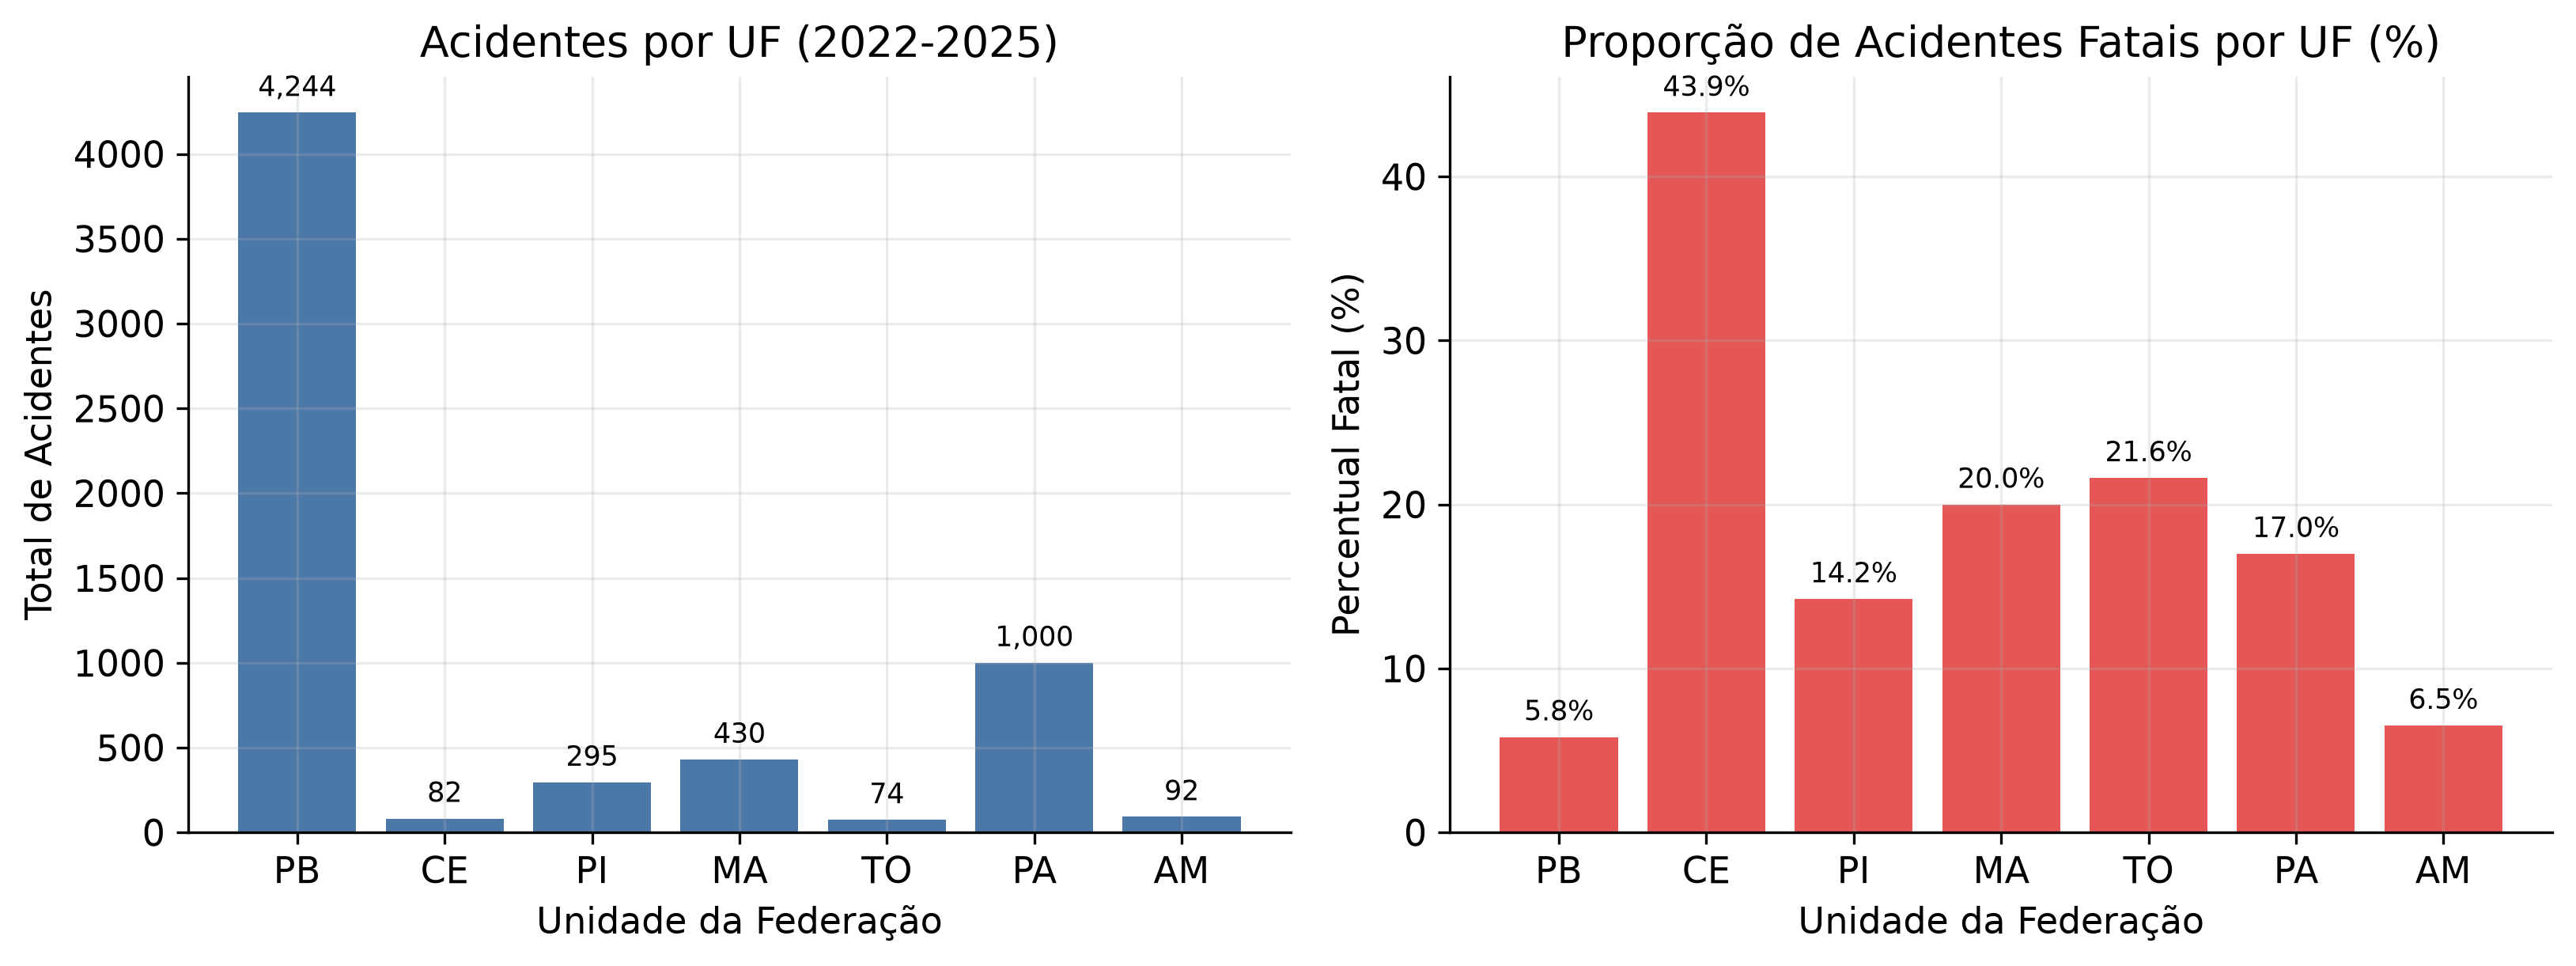
\includegraphics[width=0.92\textwidth]{figuras/acidentes_letalidade_uf.png}
\caption{Volume total de acidentes (esquerda) e taxa percentual de acidentes fatais (direita) por unidade federativa na BR-230 (2022--2025).}
\label{fig:barras_uf}
\end{figure}

\subsection{Questão 2: Padrões Temporais das Ocorrências}

\textit{Quando os acidentes acontecem? Os períodos com maior volume coincidem com os momentos de maior gravidade?}

A Figura~\ref{fig:temporal} apresenta a decomposição temporal dos acidentes em três dimensões: mensal, dia da semana e distribuição horária ao longo das 24 horas.

\begin{figure}[H]
\centering
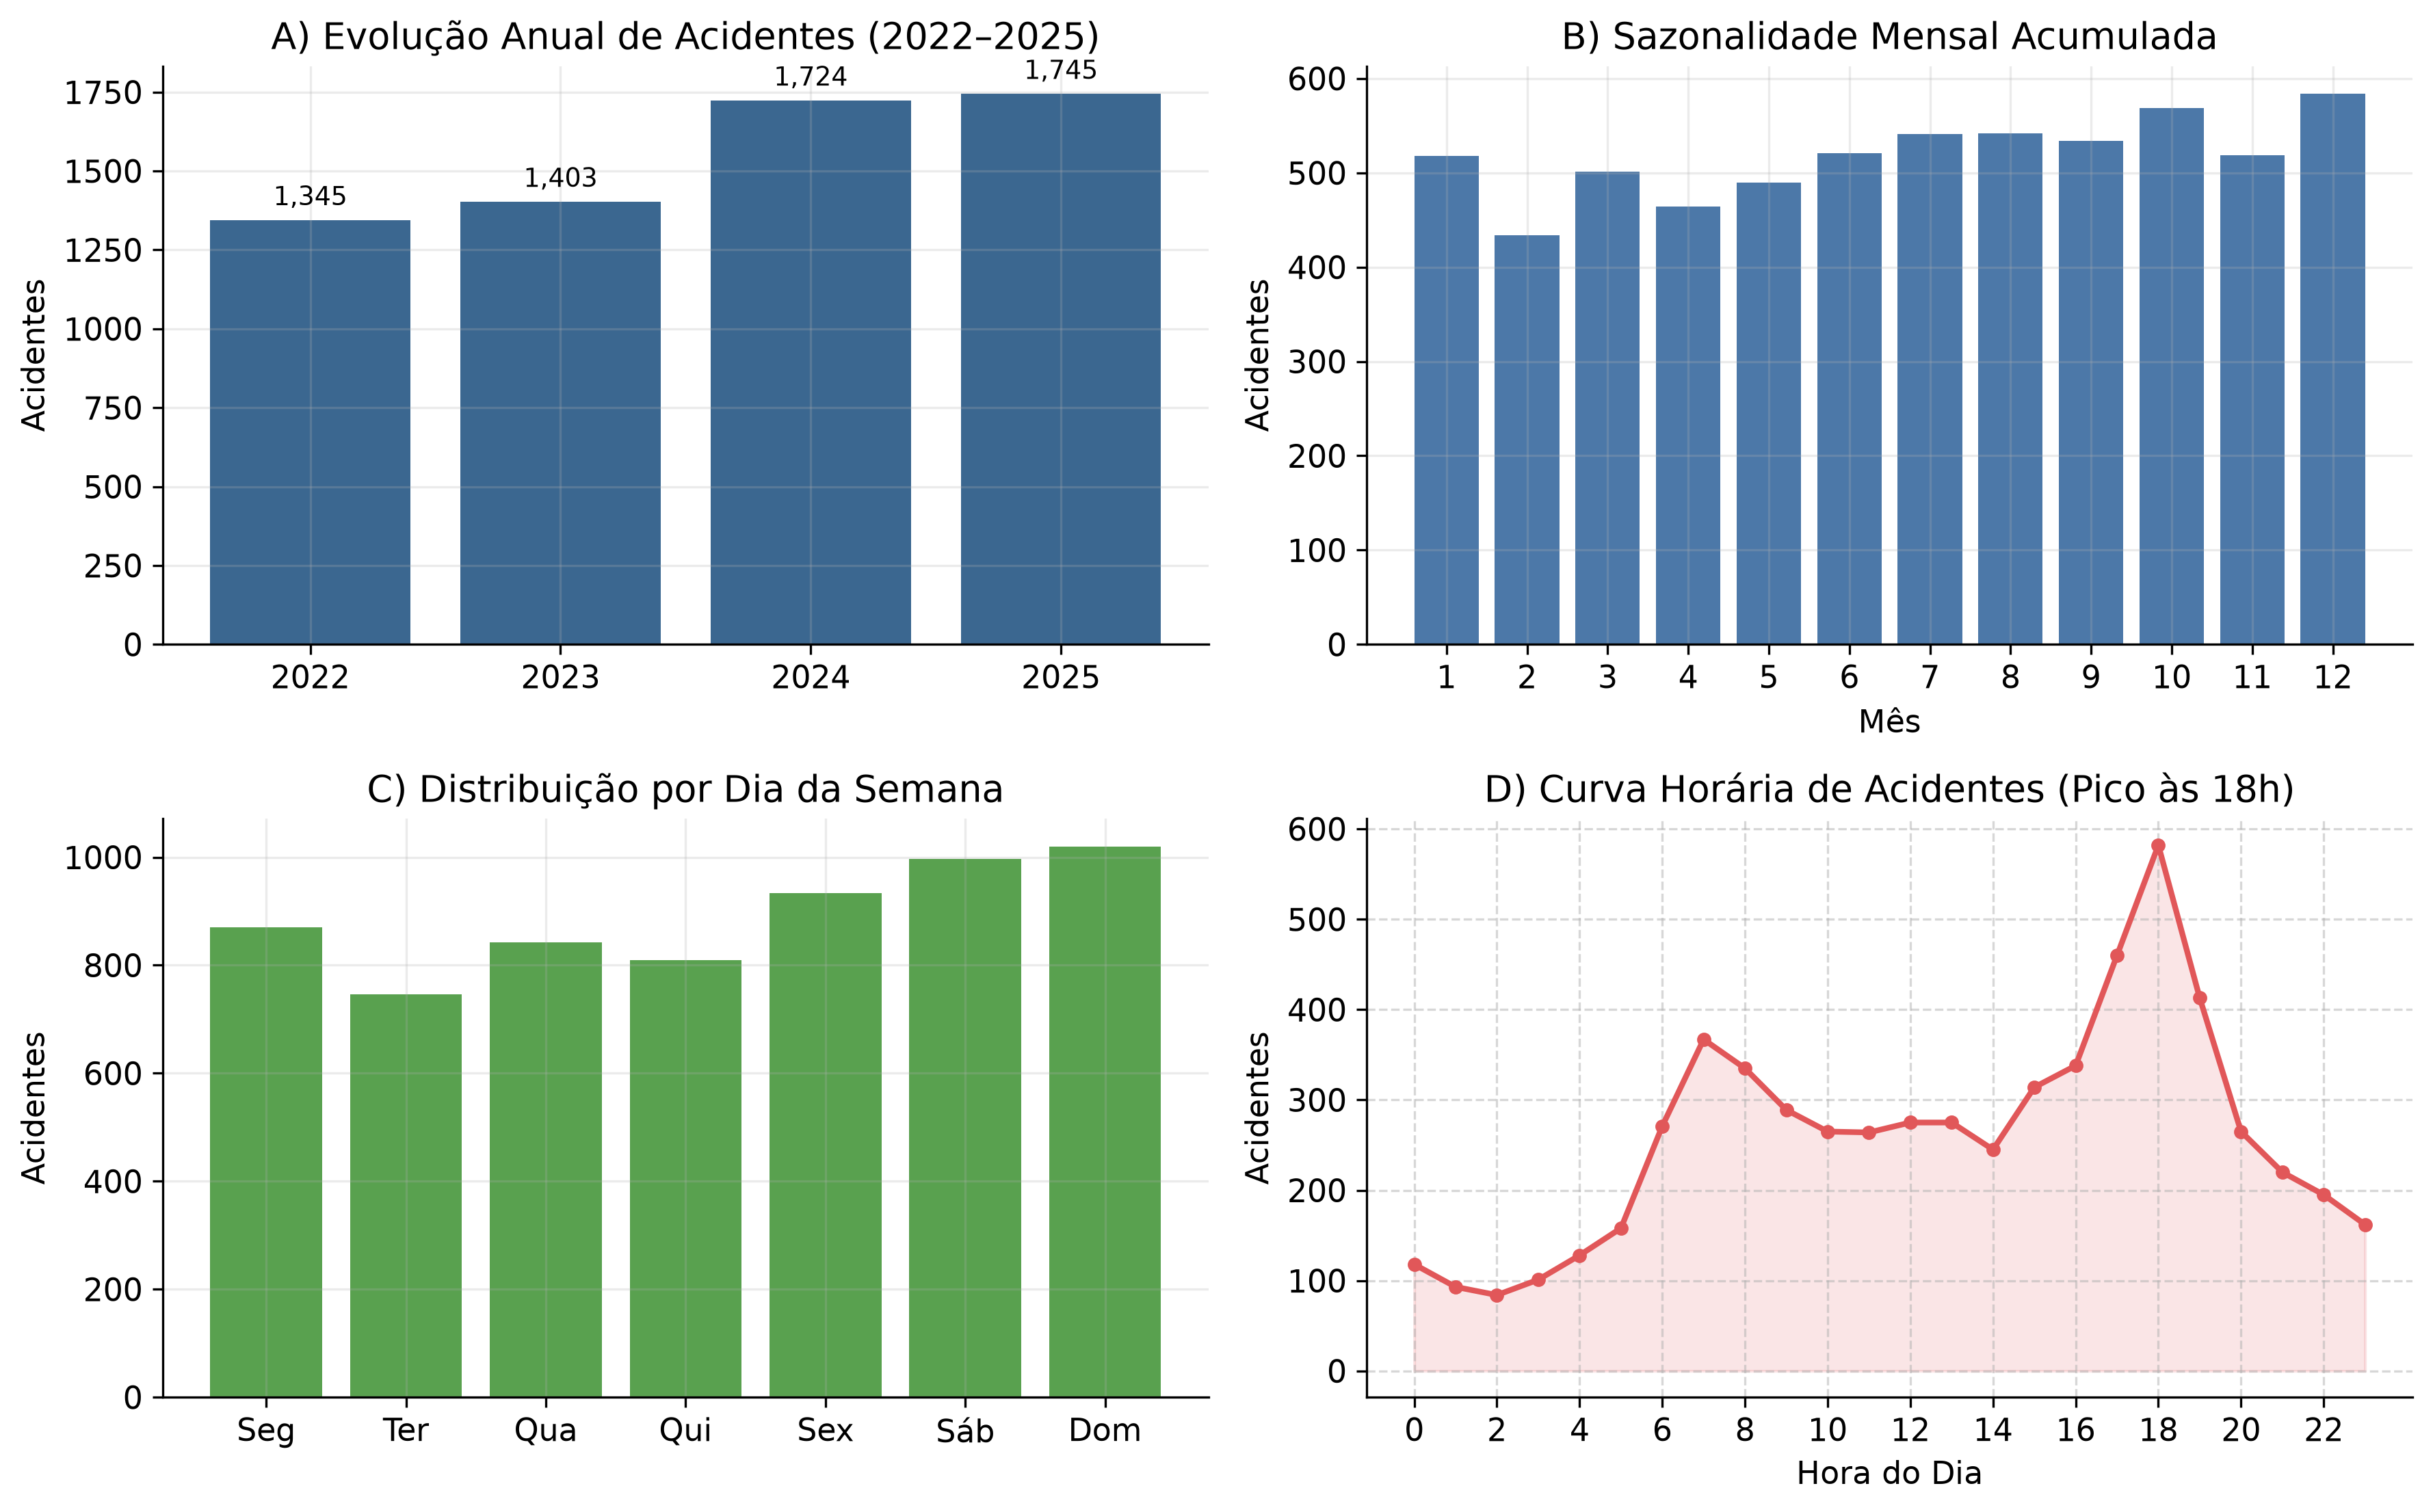
\includegraphics[width=\textwidth]{figuras/distribuicao_temporal.png}
\caption{Painel temporal consolidado da BR-230 (2022--2025): evolução anual (A), sazonalidade mensal (B), dia da semana (C) e curva horária com pico às 18h (D).}
\label{fig:temporal}
\end{figure}

\begin{itemize}
    \item \textbf{Sazonalidade Mensal:} O volume mensal consolidado no quadriênio 2022--2025 revela estabilidade rigorosa (média de 518 acidentes acumulados por mês), com ligeira elevação nos meses do segundo semestre (pico em dezembro com 578 casos).
    \item \textbf{Dia da Semana:} Notável concentração nos finais de semana: sexta-feira (933 casos; 15,0\%), sábado (997 casos; 16,0\%) e domingo (1.020 casos; 16,4\%). O \textbf{domingo} reúne a maior letalidade: \textbf{13,92\% dos acidentes resultam em óbito} (157 mortes acumuladas).
    \item \textbf{Ciclo Horário e Fase do Dia:} O pico de registros ocorre pontualmente às 18:00 (504 acidentes acumulados), coincidindo com a saída do trabalho e a transição dia-noite. Já a letalidade percentual atinge ápice na \textbf{Plena Noite (13,00\%)} e no \textbf{Amanhecer (19,15\%)}, quase o triplo do registrado em Pleno Dia (7,06\%), conforme comprovado na Figura~\ref{fig:fase_dia}.
\end{itemize}

\begin{figure}[H]
\centering
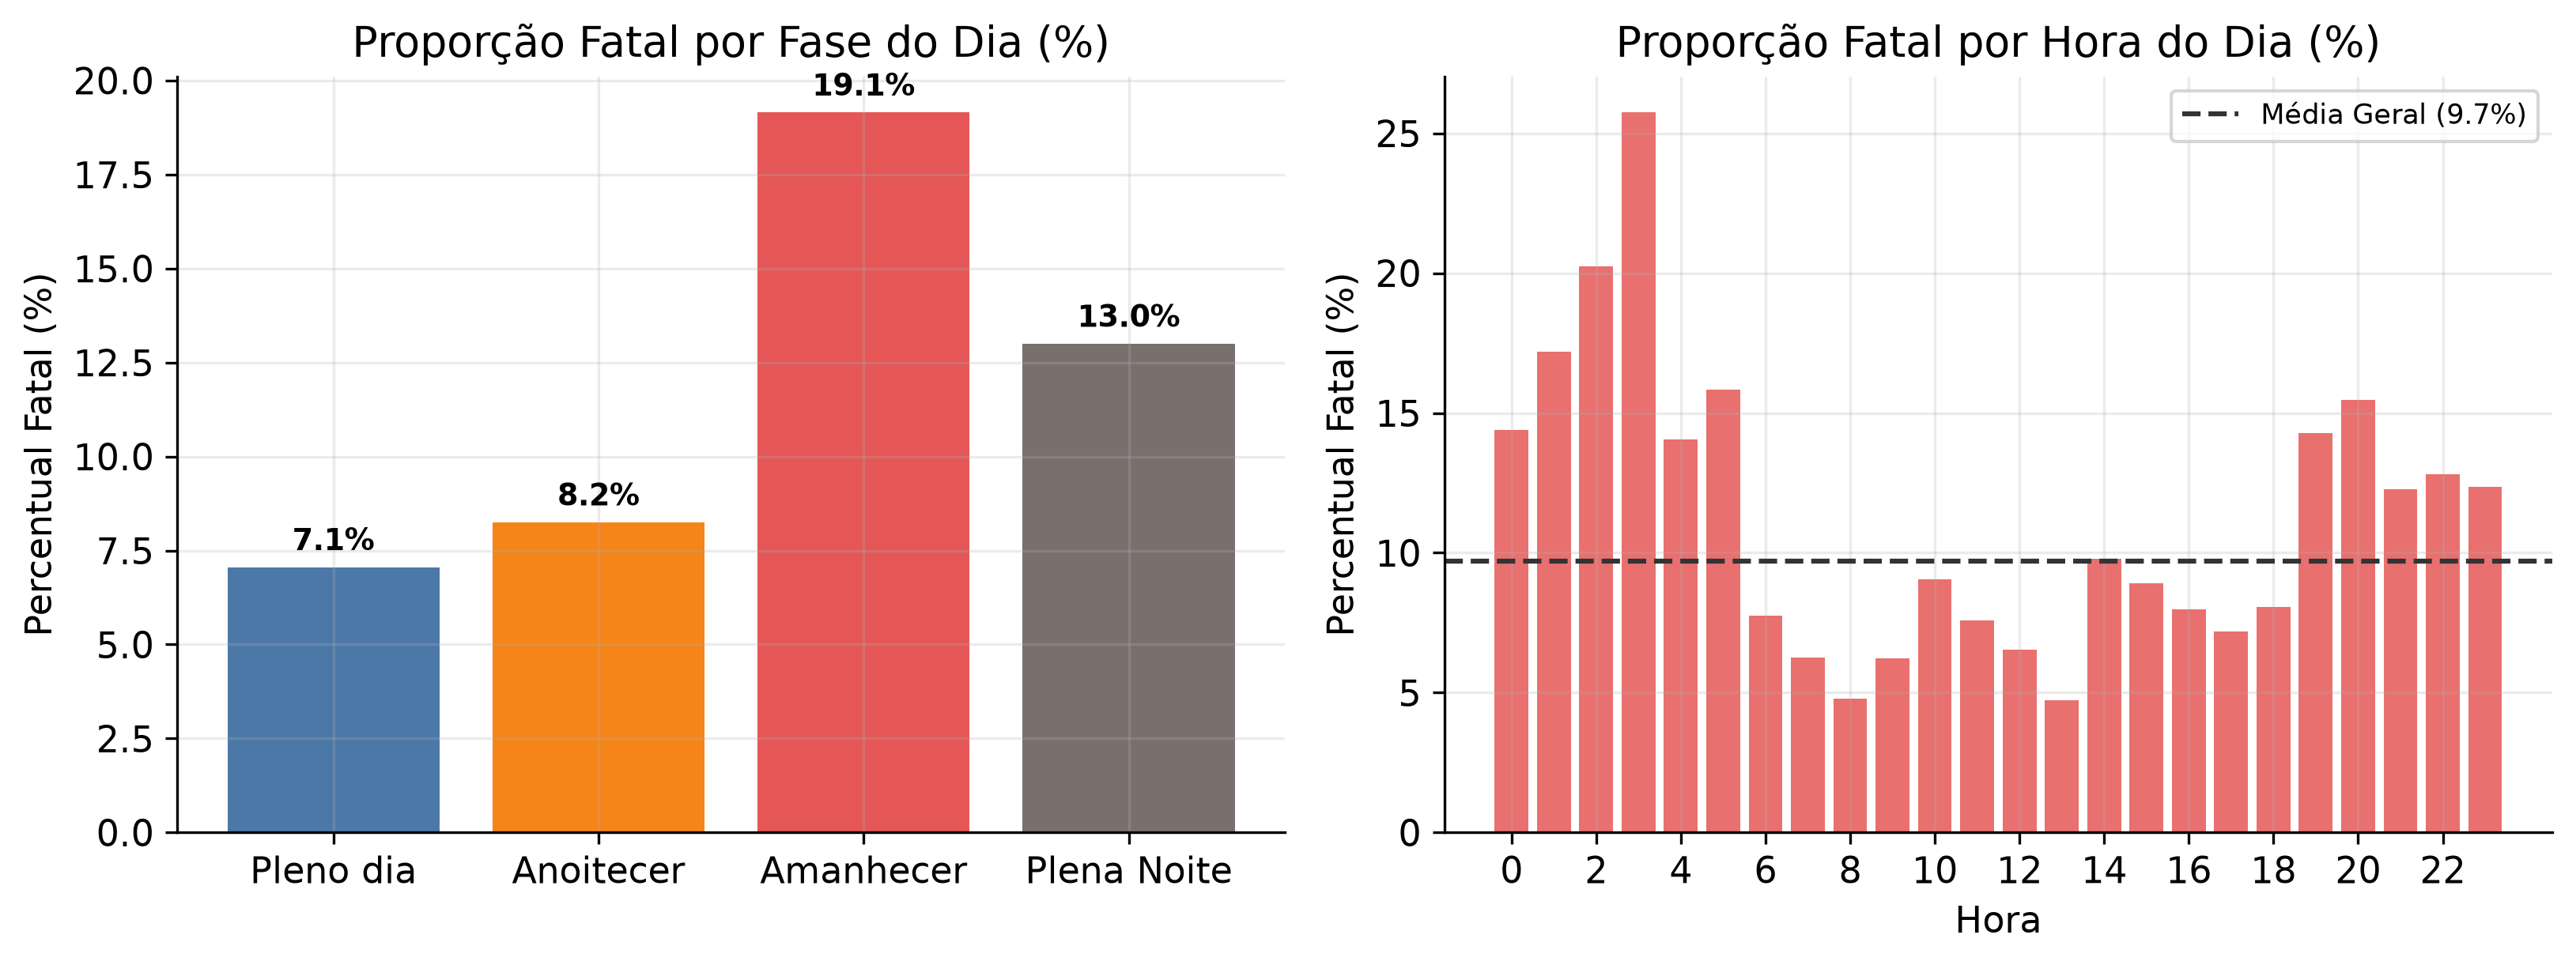
\includegraphics[width=0.82\textwidth]{figuras/fase_dia_letalidade.png}
\caption{Proporção de acidentes com vítimas fatais segundo a fase do dia (esquerda) e taxa horária (direita) na BR-230 (2022--2025).}
\label{fig:fase_dia}
\end{figure}

\subsection{Questão 3: Influência da Via, Geometria e Meteorologia}

\textit{Quais características físicas e meteorológicas se associam ao aumento do risco?}

\begin{itemize}
    \item \textbf{Condição Meteorológica:} 70,6\% dos sinistros no quadriênio ocorreram sob \textbf{Céu Claro} (4.391 casos; letalidade de 9,84\%), 10,5\% sob céu \textbf{Nublado} (650 casos; 10,62\% fatais), 7,4\% sob \textbf{Sol} (462 casos) e 6,9\% sob \textbf{Chuva} (431 casos; letalidade de 7,89\%). A menor letalidade sob chuva decorre da prudência e redução forçada de velocidade em pista molhada.
    \item \textbf{Tipo de Pista:} O volume na BR-230 divide-se entre Pista Simples (3.170 casos; 51,0\%), Pista Dupla (2.865 casos; 46,1\%) e Pista Múltipla (182 casos; 2,9\%). Todavia, a \textbf{Pista Simples concentra 76,7\% de todas as mortes da BR-230} (518 dos 675 óbitos), exibindo proporção fatal quase três vezes superior à da pista dupla (14,26\% vs. 5,06\%).
    \item \textbf{Uso do Solo:} O ambiente urbano concentra 55,3\% dos sinistros (3.439 casos; 5,61\% fatais e 202 mortes), enquanto a área rural responde por 44,7\% (2.778 casos; \textbf{14,76\% fatais} e 473 mortes acumuladas).
    \item \textbf{Geometria da Via:} Trechos em reta concentram a maioria dos registros, mas curvas em pista simples no interior destacam-se pela severidade letal.
\end{itemize}

\subsection{Questão 4: Gravidade e Variável-Alvo Preditiva}

\textit{Onde os acidentes são mais severos? Como estruturar a variável-alvo para modelagem?}

A constatação analítica mais relevante da Fase 2 é a \textbf{dissociação entre concentração de acidentes e gravidade}:
\begin{itemize}
    \item Onde os acidentes são mais volumosos (trecho metropolitano paraibano, pista dupla, urbano), a severidade percentual é baixa (3,4\% fatais).
    \item Onde os acidentes são raros e dispersos (pista simples, área rural), a gravidade dispara.
\end{itemize}

A Tabela~\ref{tab:cruzada} documenta o cruzamento entre Uso do Solo e Tipo de Pista, demonstrando que na área rural em pista simples fora da Paraíba, \textbf{25,10\% dos acidentes resultam em mortes} (1 em cada 4 acidentes é fatal).

\begin{table}[H]
\centering
\small
\renewcommand{\arraystretch}{1.2}
\caption{Cruzamento bivariado consolidado de severidade: Uso do Solo $\times$ Tipo de Pista (2022--2025).}
\label{tab:cruzada}
\begin{tabularx}{\textwidth}{|p{3.8cm}|p{2.5cm}|p{2.5cm}|c|c|c|}
\hline
\textbf{Recorte Territorial} & \textbf{Uso do Solo} & \textbf{Tipo de Pista} & \textbf{Acidentes} & \textbf{Prop. Fatais (\%)} & \textbf{Mortos} \\
\hline
BR-230 Completa & Urbano (Sim) & Dupla & 1.952 & 4,66\% & 93 \\
\hline
BR-230 Completa & Urbano (Sim) & Simples & 1.330 & 7,37\% & 105 \\
\hline
BR-230 Completa & Rural (Não) & Dupla & 913 & 5,91\% & 58 \\
\hline
\textbf{BR-230 Completa} & \textbf{Rural (Não)} & \textbf{Simples} & \textbf{1.840} & \textbf{19,24\%} & \textbf{413} \\
\hline
\hline
Fora da Paraíba & Urbano (Sim) & Simples & 540 & 11,67\% & 68 \\
\hline
Fora da Paraíba & Urbano (Sim) & Dupla & 359 & 8,08\% & 29 \\
\hline
\textbf{Fora da Paraíba} & \textbf{Rural (Não)} & \textbf{Simples} & \textbf{1.040} & \textbf{25,10\%} & \textbf{295} \\
\hline
\end{tabularx}
\end{table}

\textbf{Definição da Variável-Alvo:} Para a modelagem preditiva, estabelece-se a gravidade binária do sinistro (\texttt{Com Vítimas Fatais}). Na série consolidada 2022--2025 da BR-230, contabilizam-se \textbf{6.217 acidentes, sendo 603 fatais (9,70\%)}, acumulando 675 mortes e 7.074 feridos. Esse desbalanceamento de classes (~1:9,3) é consistente e robusto ao longo dos quatro anos, orientando as estratégias de ponderação e amostragem sintética nas Fases 3 e 4.

\subsection{Questão 5: Causas, Tipos de Sinistro, Perfil de Vítimas e Veículos}

\textit{Quais causas e dinâmicas predominam? Qual é o perfil dos indivíduos e veículos?}

\begin{itemize}
    \item \textbf{Causas Determinantes:} Ausência de reação do condutor (1.062 acidentes; 17,1\%), Reação tardia ou ineficiente do condutor (850 acidentes; 13,7\%), Acessar a via sem observar veículos (632 acidentes; 10,2\%), Condutor deixou de manter distância segura (455 acidentes; 7,3\%) e Ingestão de álcool pelo condutor (360 acidentes; 5,8\%).
    \item \textbf{Tipos de Acidente:} Colisão traseira (1.273 casos; 20,5\%), Colisão transversal (817; 13,1\%), Saída de leito carroçável (802; 12,9\%), Tombamento (765; 12,3\%), Colisão lateral (610; 9,8\%) e Colisão frontal (475 casos; 7,6\% --- modalidade responsável pela maior taxa de óbito instantâneo).
    \item \textbf{Perfil dos Envolvidos:} Dos \textbf{15.764 registros de pessoas} na BR-230 no quadriênio, os condutores totalizam 10.427 (66,1\%), passageiros 3.867 (24,5\%) e pedestres 282 (1,8\%). Nos registros com sexo informado, 74,9\% são homens (10.102) e 25,1\% mulheres (3.380). A idade dos envolvidos apresenta média de \textbf{38,4 anos} e mediana de \textbf{37,0 anos}, conforme evidenciado no histograma da Figura~\ref{fig:idade}.
    \item \textbf{Frota de Veículos:} Os automóveis totalizam 4.992 veículos (31,7\%) e as motocicletas 4.570 (29,0\%), seguidos por caminhonetes (1.521; 9,6\%) e transporte pesado de carga (caminhões, semirreboques e caminhões-trator somam 2.083 unidades; 13,2\%). A vulnerabilidade dos motociclistas e a severidade dos impactos com veículos pesados destacam-se como os fatores determinantes de óbito.
\end{itemize}

\begin{figure}[H]
\centering
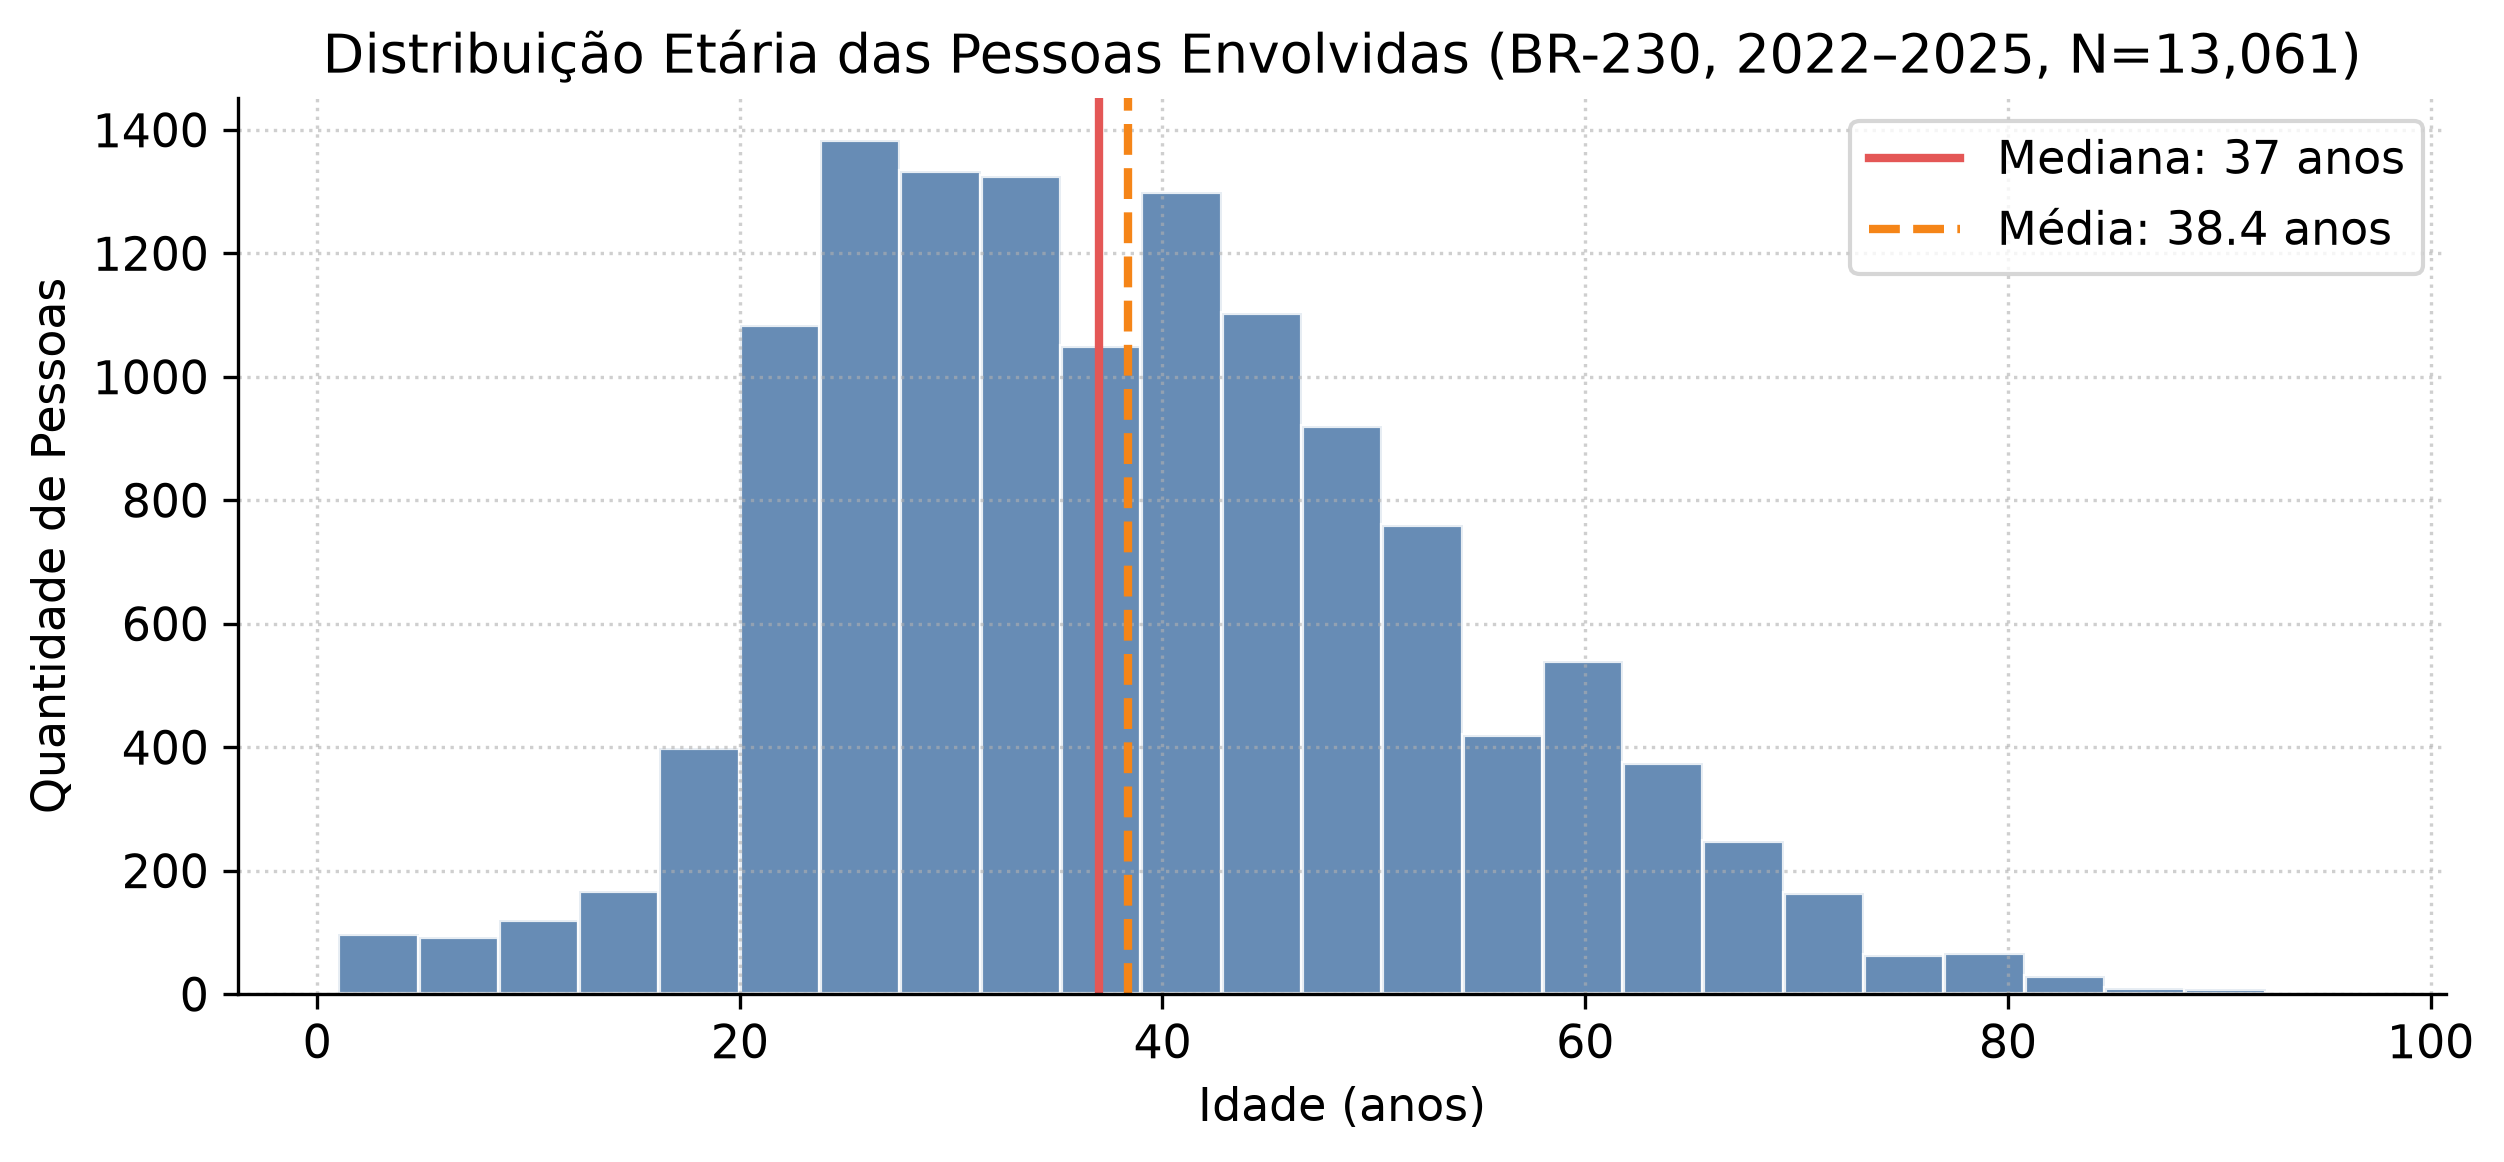
\includegraphics[width=0.75\textwidth]{figuras/distribuicao_idade.png}
\caption{Distribuição etária das pessoas envolvidas em acidentes na BR-230 em 2025.}
\label{fig:idade}
\end{figure}

\newpage

% =========================================================
% 4 QUALIDADE DOS DADOS
% =========================================================
\section{Qualidade dos Dados}

A tarefa de verificação da qualidade dos dados (\textit{Verify data quality}) avalia completude, correção, inconsistências e valores ausentes, prescrevendo encaminhamentos concretos para a Fase 3 (Preparação).

\subsection{Completude dos Dados e Limitações Estruturais}

\begin{itemize}
    \item \textbf{Completude Operacional:} A base cobre com 100\% de preenchimento as variáveis geográficas (\texttt{latitude}, \texttt{longitude}), quilômetro, data, horário e gravidade para os 1.745 acidentes da BR-230.
    \item \textbf{Limitação de Exposição (Ausência de Tráfego/VMD):} A base da PRF cobre estritamente ocorrências consumadas. Não há dados de contagem contínua de veículos (Volume Médio Diário do DNIT) nem registros de trechos-hora seguros. Consequentemente, o modelo preditivo expressa a \textbf{probabilidade condicional de gravidade} ($P(\text{Fatal} \mid \text{Acidente})$), enquanto o Mapa de Calor expressa a \textbf{densidade histórica de concentração}.
\end{itemize}

\subsection{Correção e Identificação de Erros Lógicos}

\begin{enumerate}
    \item \textbf{Código Sentinela \texttt{pesid = 0}:} Identificou-se 263 linhas com \texttt{pesid = 0} na BR-230. Trata-se de código sentinela da PRF para vítimas não identificadas ou condutores foragidos. A repetição do valor zero no mesmo boletim gerava a falsa impressão de linhas duplicadas.
    \item \textbf{Valores Sentinela em Idade e Ano:} Foram constatadas 753 linhas com \texttt{idade = 0} e 567 com \texttt{ano\_fabricacao\_veiculo = 0}, atuando como omissão e não como grandezas numéricas. Identificou-se ainda 1 registro com idade de 914 anos (erro de digitação).
    \item \textbf{Divergência Político-Administrativa:} Em 34 acidentes na divisa MA/PI, a circunscrição da PRF (SPRF-PI) difere do estado geográfico do município (MA). Estabeleceu-se que as coordenadas e o município têm prevalência absoluta sobre a unidade administrativa.
    \item \textbf{Traçados Compostos:} 536 boletins apresentam valores combinados por ponto e vírgula no campo \texttt{tracado\_via}.
\end{enumerate}

\subsection{Valores Ausentes}

A Tabela~\ref{tab:ausencias} detalha as taxas de valores nulos nos arquivos do estudo.

\begin{table}[H]
\centering
\small
\renewcommand{\arraystretch}{1.2}
\caption{Diagnóstico de valores ausentes por arquivo e atributo.}
\label{tab:ausencias}
\begin{tabularx}{\textwidth}{|p{3.5cm}|p{2.8cm}|c|X|}
\hline
\textbf{Arquivo} & \textbf{Campo} & \textbf{Nulos / Taxa} & \textbf{Diagnóstico e Impacto no Projeto} \\
\hline
\texttt{datatran2025.csv} & \texttt{uop}, \texttt{delegacia} & 38 / 22 casos (nac.) & Metadados policiais; sem impacto para o modelo. \\
\hline
\texttt{datatran2025.csv} & \texttt{lat, lon, km, data} & 0 nulos na BR-230 & Completude de 100\%; nenhum descarte espacial. \\
\hline
\texttt{acidentes2025.csv} & \texttt{tipo\_envolvido, sexo} & 8,81\% (nacional) & Omissão de dados de vítimas evadidas ou não identificadas. \\
\hline
\texttt{acidentes2025.csv} & \texttt{tipo\_veiculo} & 3,26\% (nacional) & Pedestres, animais ou veículos não cadastrados. \\
\hline
\texttt{expandido} & \texttt{idade} & 18,08\% (nacional) & Exige tratamento de sentinela e imputação na Fase 3. \\
\hline
\end{tabularx}
\end{table}

\subsection{Validação com Fontes Externas}

Confrontando os cálculos locais contra o Anuário Estatístico 2025 da PRF, todos os 9 indicadores oficiais conferiram com 100\% de exatidão (Tabela~\ref{tab:validacao}).

\begin{table}[H]
\centering
\small
\renewcommand{\arraystretch}{1.2}
\caption{Validação externa dos dados locais contra o Anuário Estatístico 2025 da PRF.}
\label{tab:validacao}
\begin{tabularx}{\textwidth}{|X|c|c|c|}
\hline
\textbf{Indicador de Controle Oficial} & \textbf{Anuário PRF 2025} & \textbf{Cálculo Base Local} & \textbf{Status da Validação} \\
\hline
Sinistros em Rodovias Federais (2025) & 72.529 & 72.529 & Exato (100\%) \\
\hline
Vítimas Fatais (Óbitos em 2025) & 6.043 & 6.043 & Exato (100\%) \\
\hline
Total de Vítimas Feridas & 83.550 & 83.550 & Exato (100\%) \\
\hline
Sinistros na Rodovia BR-101 & 13.014 & 13.014 & Exato (100\%) \\
\hline
Sinistros na Rodovia BR-116 & 11.021 & 11.021 & Exato (100\%) \\
\hline
Sinistros na Rodovia BR-040 & 3.502 & 3.502 & Exato (100\%) \\
\hline
Sinistros em Minas Gerais & 9.570 & 9.570 & Exato (100\%) \\
\hline
Sinistros em Santa Catarina & 8.186 & 8.186 & Exato (100\%) \\
\hline
Sinistros no Paraná & 7.630 & 7.630 & Exato (100\%) \\
\hline
\end{tabularx}
\end{table}

Além disso, os limites de quilômetro observados na Paraíba (516 km) e no Tocantins (144 km) permaneceram contidos nas extensões oficiais cadastradas pelo DNIT (521,0 km e 144,7 km, respectivamente).

\subsection{Matriz de Encaminhamentos para a Fase 3 (Preparação dos Dados)}

A Tabela~\ref{tab:encaminhamentos} formaliza o plano de ação técnico obrigatório para o pipeline de preparação.

\begin{table}[H]
\centering
\small
\renewcommand{\arraystretch}{1.25}
\caption{Matriz de decisões para o pipeline de Preparação dos Dados (Fase 3).}
\label{tab:encaminhamentos}
\begin{tabularx}{\textwidth}{|p{4.2cm}|p{3.5cm}|X|}
\hline
\textbf{Decisão Técnica} & \textbf{Motivação} & \textbf{Ação / Implementação} \\
\hline
1. Base única de ocorrências & Evitar inflar contagens de acidentes & Utilizar \texttt{datatran2025.csv} filtrado em \texttt{br == 230} para o mapa de calor e modelo primário. \\
\hline
2. Posicionamento por coordenadas & Quilometragem reinicia a cada UF & Mapear e espacializar exclusivamente pelo par (\texttt{latitude}, \texttt{longitude}) em formato WGS84. \\
\hline
3. Conversão de zeros sentinela & Zeros representam omissão & Converter \texttt{pesid = 0}, \texttt{idade = 0} e \texttt{ano = 0} para \texttt{NaN} antes de imputação ou codificação. \\
\hline
4. Tratamento de traçado composto & 536 casos com ponto e vírgula & Desmembrar em variáveis indicadoras binárias (\textit{one-hot}) ou selecionar geometria primária. \\
\hline
5. Prevalência geográfica & 34 conflitos de jurisdição policial & Prevalecer coordenadas e UF do município sobre a regional administrativa da PRF. \\
\hline
6. Tratamento do desbalanceamento & Apenas 9,63\% de acidentes fatais & Adotar ponderação de perdas (\textit{balanced weights}), avaliar alvo agrupado (\textit{Fatal + Grave}) e métricas PR-AUC/F1. \\
\hline
\end{tabularx}
\end{table}

\newpage

% =========================================================
% 5 REFERÊNCIAS
% =========================================================
\begin{thebibliography}{99}

\bibitem{chapman2000}
P.~Chapman, J.~Clinton, R.~Kerber, T.~Khabaza, T.~Reinartz, C.~Shearer e R.~Wirth.
\newblock \emph{{CRISP-DM} 1.0: Step-by-step data mining guide}.
\newblock CRISP-DM Consortium, 2000.
\newblock Dispon{\'i}vel em: \url{https://www.datascienceprocess.com/wp-content/uploads/2020/05/crisp-dm-guide.pdf}.

\bibitem{prfdados}
Pol{\'i}cia Rodovi{\'a}ria Federal.
\newblock Dados Abertos da {PRF} -- Acidentes de Tr{\'a}nsito.
\newblock Portal gov.br, acesso em 13/10/2026.
\newblock Dispon{\'i}vel em: \url{https://www.gov.br/prf/pt-br/acesso-a-informacao/dados-abertos/dados-abertos-da-prf}.

\bibitem{prfanuario2025}
Pol{\'i}cia Rodovi{\'a}ria Federal.
\newblock Anu{\'a}rio Estat{\'i}stico 2025 da Pol{\'i}cia Rodovi{\'a}ria Federal.
\newblock Divulgado em Maio de 2026.
\newblock Dispon{\'i}vel em: \url{https://www.gov.br/prf/pt-br/noticias/nacionais/2026/maio/prf-divulga-anuario-estatistico-de-2025-com-aumento-de-infracoes-e-reducao-de-mortes-nas-rodovias-federais}.

\bibitem{dnit2026}
Departamento Nacional de Infraestrutura de Transportes ({DNIT}).
\newblock Restaura{\c{c}}{\~a}o e Extens{\~o}es da Rodovia {BR-230}.
\newblock Portal gov.br/dnit, 2026.
\newblock Dispon{\'i}vel em: \url{https://www.gov.br/dnit/pt-br}.

\bibitem{tozetto2025}
J.~P.~Tozetto, I.~Nunes, B.~Soares, E.~T.~Albergaria, D.~R.~C.~Dias, V.~F.~S.~Mota e L.~C.~D.~Rocha.
\newblock Evaluating Segmentation and Temporal Resolution in Highway Crash Forecasting: The {BR-040} Corridor.
\newblock In \emph{Springer} (cap{\'i}tulo de livro), 2025.
\newblock DOI: \url{https://doi.org/10.1007/978-3-032-30488-9_36}.

\bibitem{santos2021}
D.~Santos, J.~Saias, P.~Quaresma e V.~B.~Nogueira.
\newblock Machine Learning Approaches to Traffic Accident Analysis and Hotspot Prediction.
\newblock \emph{Computers}, 10(12):157, 2021.
\newblock DOI: \url{https://doi.org/10.3390/computers10120157}.

\bibitem{behboudi2024}
N.~Behboudi, S.~Moosavi e R.~Ramnath.
\newblock Recent Advances in Traffic Accident Analysis and Prediction: A Comprehensive Review of Machine Learning Techniques.
\newblock \emph{arXiv preprint} arXiv:2406.13968, 2024.
\newblock Dispon{\'i}vel em: \url{https://arxiv.org/abs/2406.13968}.

\bibitem{le2020}
K.~G.~Le, P.~Liu e L.-T.~Lin.
\newblock Traffic accident hotspot identification by integrating kernel density estimation and spatial autocorrelation analysis: a case study.
\newblock \emph{International Journal of Crashworthiness}, 27(2):543--553, 2022.
\newblock DOI: \url{https://doi.org/10.1080/13588265.2020.1826800}.

\bibitem{iranmanesh2022}
M.~Iranmanesh, S.~Seyedabrishami e S.~Moridpour.
\newblock Identifying high crash risk segments in rural roads using ensemble decision tree-based models.
\newblock \emph{Scientific Reports}, 12:21324, 2022.
\newblock DOI: \url{https://doi.org/10.1038/s41598-022-24476-z}.

\bibitem{gao2024}
X.~Gao, X.~Jiang, J.~Haworth, D.~Zhuang, S.~Wang, H.~Chen e S.~Law.
\newblock Uncertainty-aware probabilistic graph neural networks for road-level traffic crash prediction.
\newblock \emph{Accident Analysis \& Prevention}, 208:107801, 2024.
\newblock DOI: \url{https://doi.org/10.1016/j.aap.2024.107801}.

\bibitem{khan2024}
A.~A.~Khan e J.~Hussain.
\newblock Utilizing {GIS} and Machine Learning for Traffic Accident Prediction in Urban Environment.
\newblock \emph{Civil Engineering Journal}, 10(6):1922--1935, 2024.
\newblock DOI: \url{https://doi.org/10.28991/CEJ-2024-010-06-013}.

\bibitem{he2025}
M.~He, G.~Meng, X.~Wu, X.~Han e J.~Fan.
\newblock Road Traffic Accident Prediction Based on Multi-Source Data -- A Systematic Review.
\newblock \emph{Promet -- Traffic\&Transportation}, 37(2):499--522, 2025.
\newblock DOI: \url{https://doi.org/10.7307/ptt.v37i2.763}.

\bibitem{jeyabharathi2026}
J.~Jeyabharathi, K.~J.~Lakshmi Prasad, K.~Karunakar, K.~Sai Charan e R.~Sasi Preetham.
\newblock {AI}-Driven Traffic Accident Prediction: Integrating Real-Time Weather, Analytics, and Machine Learning for Enhanced Road Safety.
\newblock In \emph{2026 9th International Conference on Intelligent Computing and Control Systems (ICICCS)}, p.~799--804, 2026.
\newblock DOI: \url{https://doi.org/10.1109/ICICCS67901.2026.11502769}.

\bibitem{affou2026}
H.~Affou, D.~Teso-Fz-Beto{\~n}o, U.~Fernandez-Gamiz, J.~A.~Ramos-Hernanz, D.~Caballero-Martin e J.~M.~Lopez-Guede.
\newblock Advances in Traffic Accident Prediction: A Survey of Novel Approaches.
\newblock \emph{Urban Science}, 10(7):349, 2026.
\newblock DOI: \url{https://doi.org/10.3390/urbansci10070349}.

\end{thebibliography}


\end{document}
